\documentclass{article}

%%%%% packages to import %%%%%%
\usepackage{graphicx} % Required for inserting images
\usepackage[useregional]{datetime2}
\usepackage[margin=1in]{geometry}

%%%%% title information %%%%%%
\title{CS482/495/496 Software Project Proposal: \\ 
add your tentative project title here}
\author{your name(s) here }
\date{\today}

\begin{document}
\maketitle % make title information appear here

\section{Client Information}
By sharing this client information and the rest of this document, you are stating that this client has provided this project as something they want (not something you created and asked if they wanted), and that they are interested in having you complete this project for your capstone.
% Complete the list items about your client
\begin{itemize}
    \item Client name: Eric Cui
    \item Client title: Teen league manager
    \item Client email address: lcui@loyola.edu
    \item Client employer: Loyola University Maryland
    \item How you know the client: Through our Professor
\end{itemize}

\section{Project Description}
% You must complete the following 4 subsections. The instructor will use this information to determine if your project might be feasible or not.

% Comment out the bracketed instructions as you finish subsections
\subsection{Overview}
[Add a few paragraphs describing your project succinctly. What problem are you trying to solve, what is the purpose of your project? Why does your client want this project?]

\subsection{Key Features}
[At this point you should have a basic understanding of your client's needs. List out the key features of the software system the client wants you to build.]

\subsection{Why this Project is Interesting}
[Why did you decide this project was interesting enough to you to be a capstone project? What about this project is enticing? Why should anyone care?]

\subsection{Areas of CS required}
[What subfields of computer science seem most likely to be relevant to your project? A capstone must involve multiple.]

\subsection{Potential Concerns and Questions}
[Is there any aspect of this project that makes you unsure if it will work, either due to your own interests/background, or that you aren't sure if it fits the requirements? Are there questions you have about this project that you want instructor feedback about?]

\subsection{Summary of Efforts to Find a Project}
(Not necessary for 482) [Briefly list out when/how you've discussed with this client, and if you've discussed with other clients who either didn't work out or didn't respond. If you considered a different project and it didn't work out, why didn't it work out?] 

[Most CS495 projects end here. The sections below are for CS482 and CS496 software projects].

\subsection{Comparison to Draft}
[For CS496 only, focus on highlighting the major differences between the draft proposal in CS495 and this one here. If there are no major differences, you can remove this subsection.]

\section{Requirements}

\subsection{Non-Functional Requirements}
[Non-functional requirements are just as important as functional requirements. Dont forget to specify them.]

\begin{table}[h!]
\centering
\begin{tabular}{c l c p{9cm}}
\hline
\textbf{ID} & \textbf{NFR Title} & \textbf{Category} & \textbf{Description} \\
\hline
NFR1 & Color Scheme & Visual/Design & The color scheme for the app should be a blue \\ \hline
NFR2 & Permission & Access & Invite/login in and out system \\ \hline
NFR3 & Security & Protection & Verification/Accounts \\ \hline
NFR4 & Managing & Updating  & changing and adding things  \\ \hline
NFR5 & Viewing & Security & Being able to use the website \\ \hline
\end{tabular}
\caption{Non-Functional requirements}
\end{table}


\subsection{Functional Requirements (User Stories)}
[In CS482, all functional requirements are written as User Stories. In CS496, some projects may use a different template to write the requirements. The table below is an example of writing the Stories. Adapt accordingly to different templates or if you want to display more info.]
\newpage

\begin{table}[h!]
\centering
\begin{tabular}{c l c p{10cm}}
\hline
\textbf{ID} & \textbf{Story Title} & \textbf{Points} & \textbf{Description} \\
\hline
A4 & Managing Teens account & 55 & As an Adult, I want to be able to watch and manage my kids/teens accounts, so that I can look and accept any invites while also seeing what they're doing on there accounts \\ \hline
A11 & Live Scores & 2584 & As an Admin, I want to be able to update live scores, so that I can keep viewers up to date on live matches 
\\ \hline
A16 & Full Match Control & 377 & As an Admin, I want to be able to check each match in the brackets, so that I can make sure everything is good to start the match and to allow teams enter 
\\ \hline
AD1 & Calender control & 610 & As an Admin, I want to be able to add matches and change/edit the bracket date so that I can updated recent changes on the calender/matches 
\\ \hline
G2 & Guest view & 2 & As a Guest, I want a way for visitors just to view whats on the website, so that they can see whats going on without having to login in or sign up \\ \hline
G9 & Profile viewing & 3 & As a Guest, I want to be able to look at others profiles, so that I can see who is who and the stats they have. 
\\ \hline
TM5 & Invite System & 233 & As a Team Manager, I want to invite members to a team, so that I can have a soccer team of 11 or more 
\\ \hline
TM6 & Posting Team Info & 89 & As a Team Manager, I want to manage the team I have, so that I can update/change whats going on with the team
\\ \hline
U3 & Login in/sign up screen & 21 & For all users (except Guest), I want to be able to sign up or login into the site with an account, so that I can save my data and be able to join/work on a team
\\ \hline
U7 & Home screen & 1597 & As a user, For all users , I want to see post and live matches, so that I can look at the current score/results while also interacting with post 
\\ \hline
U8 & Using Posts & 987 & For all users (with exceptions), I want to be able to interact with posts, so that I can like/dislike and comment on post while also know that teens cant see flagged post
\\ \hline
U12 & Watching History & 8 & For all users (except Guest), I want to be able to see the history of games I have played in or watched, so that I can have memories of what I have done or seen
\\ \hline
U13 & Profile management & 34 & For all users (except Guest), I want to be able to go into my own profile, so that I can change my info and description about me
\\ \hline
U14 & Leaving the site & 1 & For all users, I want to be able to logout of the website (or leave the website as a guest) on my account, so that I can switch accounts or not have my account open. 
\\ \hline
U15 & Full Match display & 144 & For all users, I want to be able to see time, date, place, teams competing, type (normal, playoff, final), so that I can keep with the recent results of a match
\\ \hline
U17 & Website Design & 5 & For all users, I want to be able navitgate the website , so that It can be user friendly while having a good design
\\ \hline


\end{tabular}
\caption{Functional requirements as User Stories.}
\end{table}

\section{System Design}

\subsection{Architecture}
We will be using a Model-View-Controller (MVC) architecture since the Rails API is designed to support MVC. Frontend will utilize react, backend is using Redis and MongoDB, while the Rails API handles all the endpoints and logic.\\
Potential Main Modules:
\begin{itemize}
    \item User Management Module
    \item Team Management Module
    \item League Management Module
    \item Analytics Module
    \item Admin Panel Module
    \item Notification Module
\end{itemize}

\subsection{Diagrams}
[CS482, on sprints/iterations 2-3, you need to create and update a diagram (check the assignment for which type of diagram). On CS496, since before sprint/iteration 1 you should have a class diagram and keep it up-to-date.]

\subsection{Technology}
\begin{table}[h!]
\centering
\begin{tabular}{|l|l|p{8cm}|}
\hline
\textbf{Tech} & \textbf{Type} & \textbf{Usage} \\ \hline
Ruby & Language & Backend \\ \hline
Rails & Framework & Web application framework \\ \hline
Docker & Containerizer & Containerize the app for consistency \\ \hline
Redis & RAM-Based Database & Quick data retrieval and updates; ideal for real-time data \\ \hline
React & UI Framework & Used for UI design and implementation \\ \hline
MongoDB & Schema-Based Database & Long-term data storage; performance not critical \\ \hline
RSpec & Testing tool & Used to test ruby code\\ \hline
\end{tabular}
\caption{Technologies used in the project}
\label{tab:technologies}
\end{table}

\subsection{Coding Standards}
\subsubsection{Naming}

\begin{itemize}
    \item \textbf{Global Variables:} All caps and underscores for spaces.  
    Examples: \texttt{VARIABLE}, \texttt{TEST}, \texttt{MIN\_NUM}
    
    \item \textbf{Classes:} Capitalized and CamelCase.  
    Examples: \texttt{Class}, \texttt{ClassGuide}, \texttt{ExTwo}
    
    \item \textbf{Functions:} Lowercase with underscores for spaces. Avoid using numbers.  
    Examples: \texttt{function}, \texttt{function\_two}, \texttt{print\_all\_one}
    
    \item \textbf{Variables:} Same as functions, but numbers do not require underscores.  
    Examples: \texttt{n}, \texttt{x}, \texttt{x2}, \texttt{print\_status}
    
    \item \textbf{Files:} File names should be descriptive and follow variable naming rules unless another convention is necessary.  
    Examples: \texttt{test\_file.txt}, \texttt{grid\_layout.py}, \texttt{App.jsx}
    
    \item \textbf{Folders:} Same as files. Keep names general and simple.  
    Examples: \texttt{folder}, \texttt{folder\_two}, \texttt{src}
\end{itemize}

\subsubsection{Code Formatting}

\begin{itemize}
    \item Include a blank line between each function.
    \item Use consistent and readable loop structures.
    \item Place comments above functions and significant code blocks.
    \item Inline comments should be aligned to the right of the code line they describe.
    \item Maintain consistency throughout the codebase.
\end{itemize}

\subsubsection{Commenting Rules}

\begin{itemize}
    \item Comments must be placed above each function explaining its purpose.
    \item Comments must be placed above each class.
    \item Comments should be detailed and easy to understand.
    \item Inline comments (for specific lines) must appear to the right of that line.
    \item Comments for code blocks should be placed above the block and explain its function.
    \item Create and follow standard templates for class and function comments.
\end{itemize}

\subsubsection{Coding Principles}

\begin{itemize}
    \item Follow the \textbf{DRY (Don't Repeat Yourself)} principle when designing code.
\end{itemize}
\subsubsection{Testing}
    \begin{itemize}
    \item Only allow code with unit tests and with at least 65\% coverage to be committed.
\end{itemize}

\subsection{Data}
\subsection{Data}
Our data will be in MongoDB. Below is the Entity-Relationship list that we will implement to the database:
\begin{itemize}
    \item \textbf{Entity: Admin}
        \begin{itemize}
            \item Attributes:
                \begin{itemize}
                    \item Name
                    \item Username
                    \item Password
                \end{itemize}
            \item Relationships:
                \begin{itemize}
                    \item MODIFY Teams, Profiles, Matches, Posts, and Calendar
                    \item Can RATE Matches and Posts
                    \item Can COMMENT on Posts
                \end{itemize}
        \end{itemize}
    \item \textbf{Entity: Team Manager}
        \begin{itemize}
            \item Attributes:
                \begin{itemize}
                    \item Name
                    \item Username
                    \item Password
                    \item Team
                \end{itemize}
            \item Relationships:
                \begin{itemize}
                    \item INVITE Profiles
                    \item ADD a Team
                    \item VIEW Teams, Profiles, and Calendar
                    \item Can RATE Matches and Posts
                    \item Can COMMENT on Posts
                \end{itemize}
        \end{itemize}
    \item \textbf{Entity: Adult}
        \begin{itemize}
            \item Attributes:
                \begin{itemize}
                    \item Name
                    \item Username
                    \item Password
                    \item Team
                    \item Children
                \end{itemize}
            \item Relationships:
                \begin{itemize}
                    \item ACCEPT INVITES from Team Manager
                    \item ACCEPT INVITES to their Teen from Team Manager
                    \item VIEW Teams, Profiles, and Calendar
                    \item Can RATE Matches and Posts
                    \item Can COMMENT on Posts
                \end{itemize}
        \end{itemize}
    \item \textbf{Entity: Teen}
        \begin{itemize}
            \item Attributes:
                \begin{itemize}
                    \item Name
                    \item Username
                    \item Password
                    \item Team
                    \item Adult Supervisor
                \end{itemize}
            \item Relationships:
                \begin{itemize}
                    \item CHILD OF a Adult
                    \item VIEW Teams, Profiles, and Calendar
                    \item Can RATE Matches and Posts
                    \item Can COMMENT on Posts
                \end{itemize}
        \end{itemize}
    \item \textbf{Entity: Guest}
        \begin{itemize}
            \item Relationships:
                \begin{itemize}
                    \item VIEW Matches, Teams, Profiles, Posts and Calendar
                \end{itemize}
        \end{itemize}
    \item \textbf{Entity: Team}
        \begin{itemize}
            \item Attributes:
                \begin{itemize}
                    \item Players
                    \item Team Name
                    \item Team Logo
                    \item Team Manager
                \end{itemize}
        \end{itemize}
    \item \textbf{Entity: Match}
        \begin{itemize}
            \item Attributes:
                \begin{itemize}
                    \item Score
                    \item Teams
                    \item Rating
                    \item Comments
                    \item History
                \end{itemize}
            \item Relationships:
                \begin{itemize}
                    \item Can VIEW a Team
                \end{itemize}
        \end{itemize}
    \item \textbf{Entity: Calendar}
        \begin{itemize}
            \item Attributes:
                \begin{itemize}
                    \item Matches
                \end{itemize}
            \item Relationships:
                \begin{itemize}
                    \item VIEWS Matches
                \end{itemize}
        \end{itemize}
    \item \textbf{Entity: Profile}
        \begin{itemize}
            \item Attributes:
                \begin{itemize}
                    \item Name
                    \item Team Name
                \end{itemize}
        \end{itemize}
    \item \textbf{Entity: Post}
        \begin{itemize}
            \item Attributes:
                \begin{itemize}
                    \item Comment
                    \item Reactions
                \end{itemize}
        \end{itemize}
\end{itemize}

\subsection{UI Mocks}
\begin{figure}[h]
    \centering
    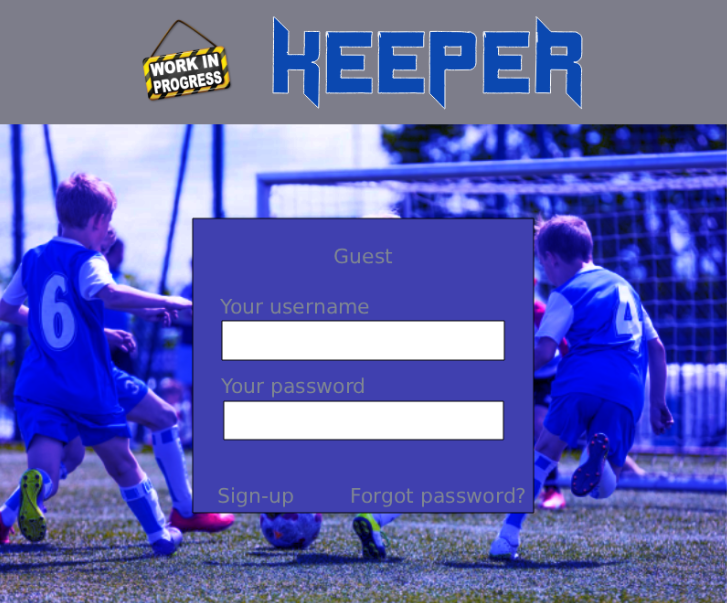
\includegraphics[width=0.6\textwidth]{images/Loginscreen .png}
    \caption{login screen with the ability to sign up or reset your password (plus being able to be a guest)}
\end{figure}

\begin{figure}[h]
    \centering
    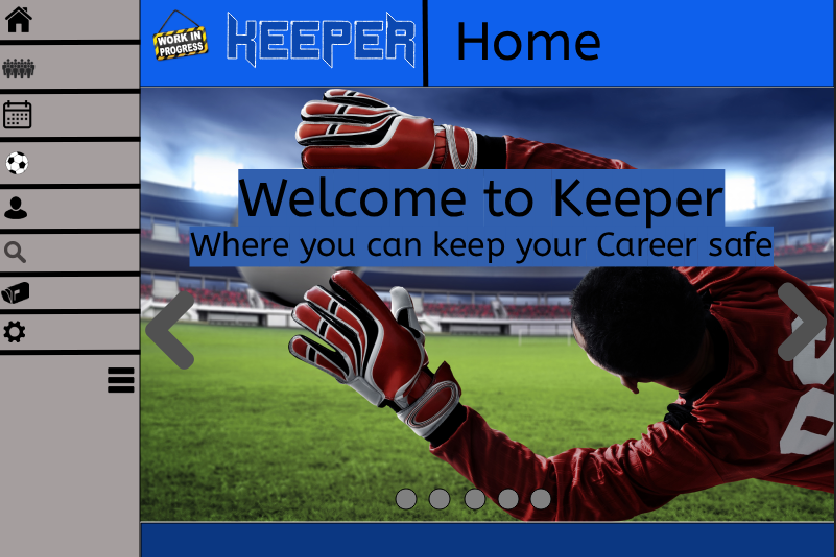
\includegraphics[width=0.6\textwidth]{images/Homescreen.png}
    \caption{Once you log in or join as a guest, you'll start from the home screen with the option bar on the left}
\end{figure}

\begin{figure}[]
    \centering
    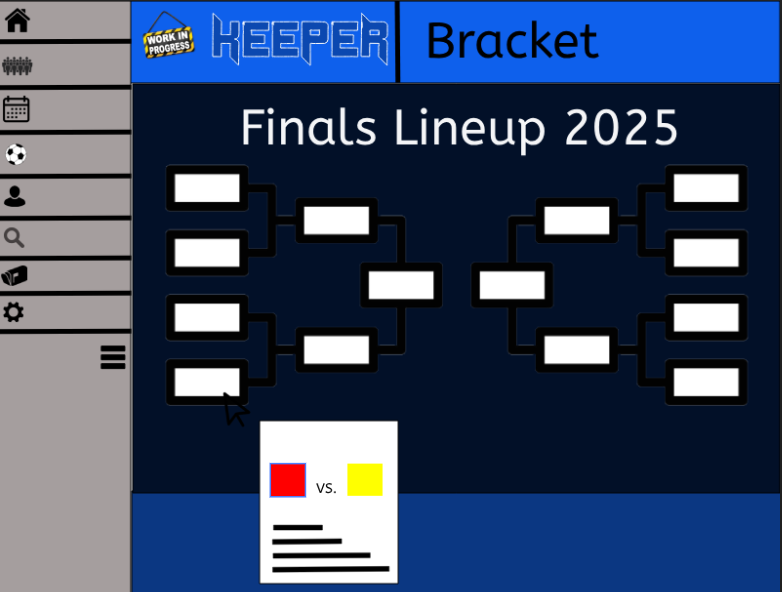
\includegraphics[width=0.5\textwidth]{images/Bracket.png}
    \caption{This is where you can see the current tournament matches that are happening while being able to click to see the info of the two teams.}
\end{figure}


\section{Iterations}

\subsection{Iteration Planning}
[In CS496, you plan all iterations beforehand. In CS482, you update the planning here at each iteration. ]

\begin{table}[h!]
\centering
\begin{tabular}{c l p{7cm} c}
\hline
\textbf{Iteration} & \textbf{Dates} & \textbf{Stories} & \textbf{Points} \\
\hline
1 & 01/01 - 02/01 & S1 Story Example, S2 Story Example 2 & 07 \\ \hline
2 & 02/01 - 03/01 & S3 Story Title, S4 Story Title, S5 Story Title, S6 Story Title & 17 \\ \hline
3 & 03/01 - 04/01 & S7 Story Title, S8 Story Title, S9 Story Title, S10 Story Title, S11 Story Title & 21 \\ \hline
4 & 04/01 - 05/01 & S12 Story Title, S13 Story Title, S14 Story Title, S15 Story Title & 19 \\ \hline
5 & 05/01 - 06/01 & S16 Story Title, S17 Story Title & 06 \\ \hline
\multicolumn{3}{r}{\bf Total: } & 70 \\ \hline
\end{tabular}
\caption{Iteration Planning for Incremental Deliveries}
\end{table}

\subsection{Iteration/Sprint 1}
\subsubsection{Planning}
[Which stories did you plan for this iteration/sprint. Add the total points for this plan. You can also explain the reason behind your planning, and what major feature(s) your team is focusing on delivering by completing these stories. You may use a table for a summary display of the planning, but elaborate in text more detail in your focus and feature plan.]

\subsubsection{Work Done}
[Which stories did you complete in this iteration/sprint. Which ones did you partially complete? Who worked on which story? You may elaborate in paragraph(s) to add more detail about the work done.]

\subsubsection{Testing Coverage}
[Testing is very important. Show your coverage here. Is this coverage good enough? Explain why you think so. Is it not good enough? Explain a plan to increase the coverage. You may also elaborate on why some artifacts do not undergo much testing. If the testing changed from the last iteration, explain the reasons.]

\subsubsection{Retroespective \& Reflection}
[What were the pitfalls, challenges, and issues you had in this iteration? How can you address them to improve the process in the next iteration? Did anything not go according to plan? Why so and how to avoid the same mistake? Write a personal reflection on what you learned in this iteration (even if a small technical thing like Database storage).]


\subsection{Iteration/Sprint 2}
\subsubsection{Planning}
[Which stories did you plan for this iteration/sprint. Add the total points for this plan. You can also explain the reason behind your planning, and what major feature(s) your team is focusing on delivering by completing these stories. You may use a table for a summary display of the planning, but elaborate in text more detail in your focus and feature plan.]

\subsubsection{Work Done}
[Which stories did you complete in this iteration/sprint. Which ones did you partially complete? Who worked on which story? You may elaborate in paragraph(s) to add more detail about the work done.]

\subsubsection{Testing Coverage}
[Testing is very important. Show your coverage here. Is this coverage good enough? Explain why you think so. Is it not good enough? Explain a plan to increase the coverage. You may also elaborate on why some artifacts do not undergo much testing. If the testing changed from the last iteration, explain the reasons.]

\subsubsection{Retroespective \& Reflection}
[What were the pitfalls, challenges, and issues you had in this iteration? How can you address them to improve the process in the next iteration? Did anything not go according to plan? Why so and how to avoid the same mistake? Write a personal reflection on what you learned in this iteration (even if a small technical thing like Database storage).]

\subsection{Iteration/Sprint 3}
\subsubsection{Planning}
[Which stories did you plan for this iteration/sprint. Add the total points for this plan. You can also explain the reason behind your planning, and what major feature(s) your team is focusing on delivering by completing these stories. You may use a table for a summary display of the planning, but elaborate in text more detail in your focus and feature plan.]

\subsubsection{Work Done}
[Which stories did you complete in this iteration/sprint. Which ones did you partially complete? Who worked on which story? You may elaborate in paragraph(s) to add more detail about the work done.]

\subsubsection{Testing Coverage}
[Testing is very important. Show your coverage here. Is this coverage good enough? Explain why you think so. Is it not good enough? Explain a plan to increase the coverage. You may also elaborate on why some artifacts do not undergo much testing. If the testing changed from the last iteration, explain the reasons.]

\subsubsection{Retroespective \& Reflection}
[What were the pitfalls, challenges, and issues you had in this iteration? How can you address them to improve the process in the next iteration? Did anything not go according to plan? Why so and how to avoid the same mistake? Write a personal reflection on what you learned in this iteration (even if a small technical thing like Database storage).]

\subsection{Iteration/Sprint 4}
[CS496 has 5 sprints. CS482 only has only 3 sprints (remove Iterations 4 and 5 from this doc if you are writing a doc for 482]

\subsubsection{Planning}
[Which stories did you plan for this iteration/sprint. Add the total points for this plan. You can also explain the reason behind your planning, and what major feature(s) your team is focusing on delivering by completing these stories. You may use a table for a summary display of the planning, but elaborate in text more detail in your focus and feature plan.]

\subsubsection{Work Done}
[Which stories did you complete in this iteration/sprint. Which ones did you partially complete? Who worked on which story? You may elaborate in paragraph(s) to add more detail about the work done.]

\subsubsection{Testing Coverage}
[Testing is very important. Show your coverage here. Is this coverage good enough? Explain why you think so. Is it not good enough? Explain a plan to increase the coverage. You may also elaborate on why some artifacts do not undergo much testing. If the testing changed from the last iteration, explain the reasons.]

\subsubsection{Retroespective \& Reflection}
[What were the pitfalls, challenges, and issues you had in this iteration? How can you address them to improve the process in the next iteration? Did anything not go according to plan? Why so and how to avoid the same mistake? Write a personal reflection on what you learned in this iteration (even if a small technical thing like Database storage).]

\subsection{Iteration/Sprint 5}
\subsubsection{Planning}
[Which stories did you plan for this iteration/sprint. Add the total points for this plan. You can also explain the reason behind your planning, and what major feature(s) your team is focusing on delivering by completing these stories. You may use a table for a summary display of the planning, but elaborate in text more detail in your focus and feature plan.]

\subsubsection{Work Done}
[Which stories did you complete in this iteration/sprint. Which ones did you partially complete? Who worked on which story? You may elaborate in paragraph(s) to add more detail about the work done.]

\subsubsection{Testing Coverage}
[Testing is very important. Show your coverage here. Is this coverage good enough? Explain why you think so. Is it not good enough? Explain a plan to increase the coverage. You may also elaborate on why some artifacts do not undergo much testing. If the testing changed from the last iteration, explain the reasons.]

\subsubsection{Retroespective \& Reflection}
[What were the pitfalls, challenges, and issues you had in this iteration? How can you address them to improve the process in the next iteration? Did anything not go according to plan? Why so and how to avoid the same mistake? Write a personal reflection on what you learned in this iteration (even if a small technical thing like Database storage).]

\section{Final Remarks}

\subsection{Overall Progress}
[Have you completed everything? If so, present evidence on how you brought value to your client, and the overall client satisfaction. Otherwise, estimate how much progress you done and how long it would take to finish this project.]

\subsection{Project Reflection}
[Your personal reflection on the project. What lessons did you learned. What would you have done differently. How can you do better work in future projects? You may write this as a team or per person (or both)]

\section*{Appendix}
[Appendix section if needed]


\end{document}
